% =============================================================================
% CHAPITRE 3 — CONCEPTION ET ARCHITECTURE DE LA SOLUTION DROPPY
% =============================================================================

\chapter{Conception et architecture de la solution Droppy}

% =============================================================================
% 3.1 INTRODUCTION
% =============================================================================

\section{Introduction}

Après l'analyse des besoins présentée dans le chapitre précédent, cette étape
consiste à concevoir la solution Droppy et à définir son architecture.

La conception est présentée à travers plusieurs vues complémentaires permettant
de représenter le système sous différents angles : fonctionnel, architectural,
dynamique, statique et physique.

Les modèles retenus sont le diagramme de cas d'utilisation, l'architecture
globale, deux diagrammes de séquence, le diagramme de classes et le diagramme
de déploiement.


% =============================================================================
% 3.2 ARCHITECTURE GLOBALE
% =============================================================================

\section{Architecture globale}

Droppy repose sur une architecture distribuée organisée autour de trois
composants principaux : une application web Angular 19, un Core Service
Spring Boot 3 et un microservice d'intelligence artificielle développé avec
FastAPI.

Le Core Service constitue le point central de communication entre l'interface
utilisateur, le service d'intelligence artificielle et la base de données.
L'application Angular communique avec Spring Boot à travers des API REST et
un canal WebSocket pour les notifications en temps réel. Spring Boot
communique quant à lui avec le microservice FastAPI pour les opérations de
détection et de prévision.

\begin{figure}[H]
    \centering
    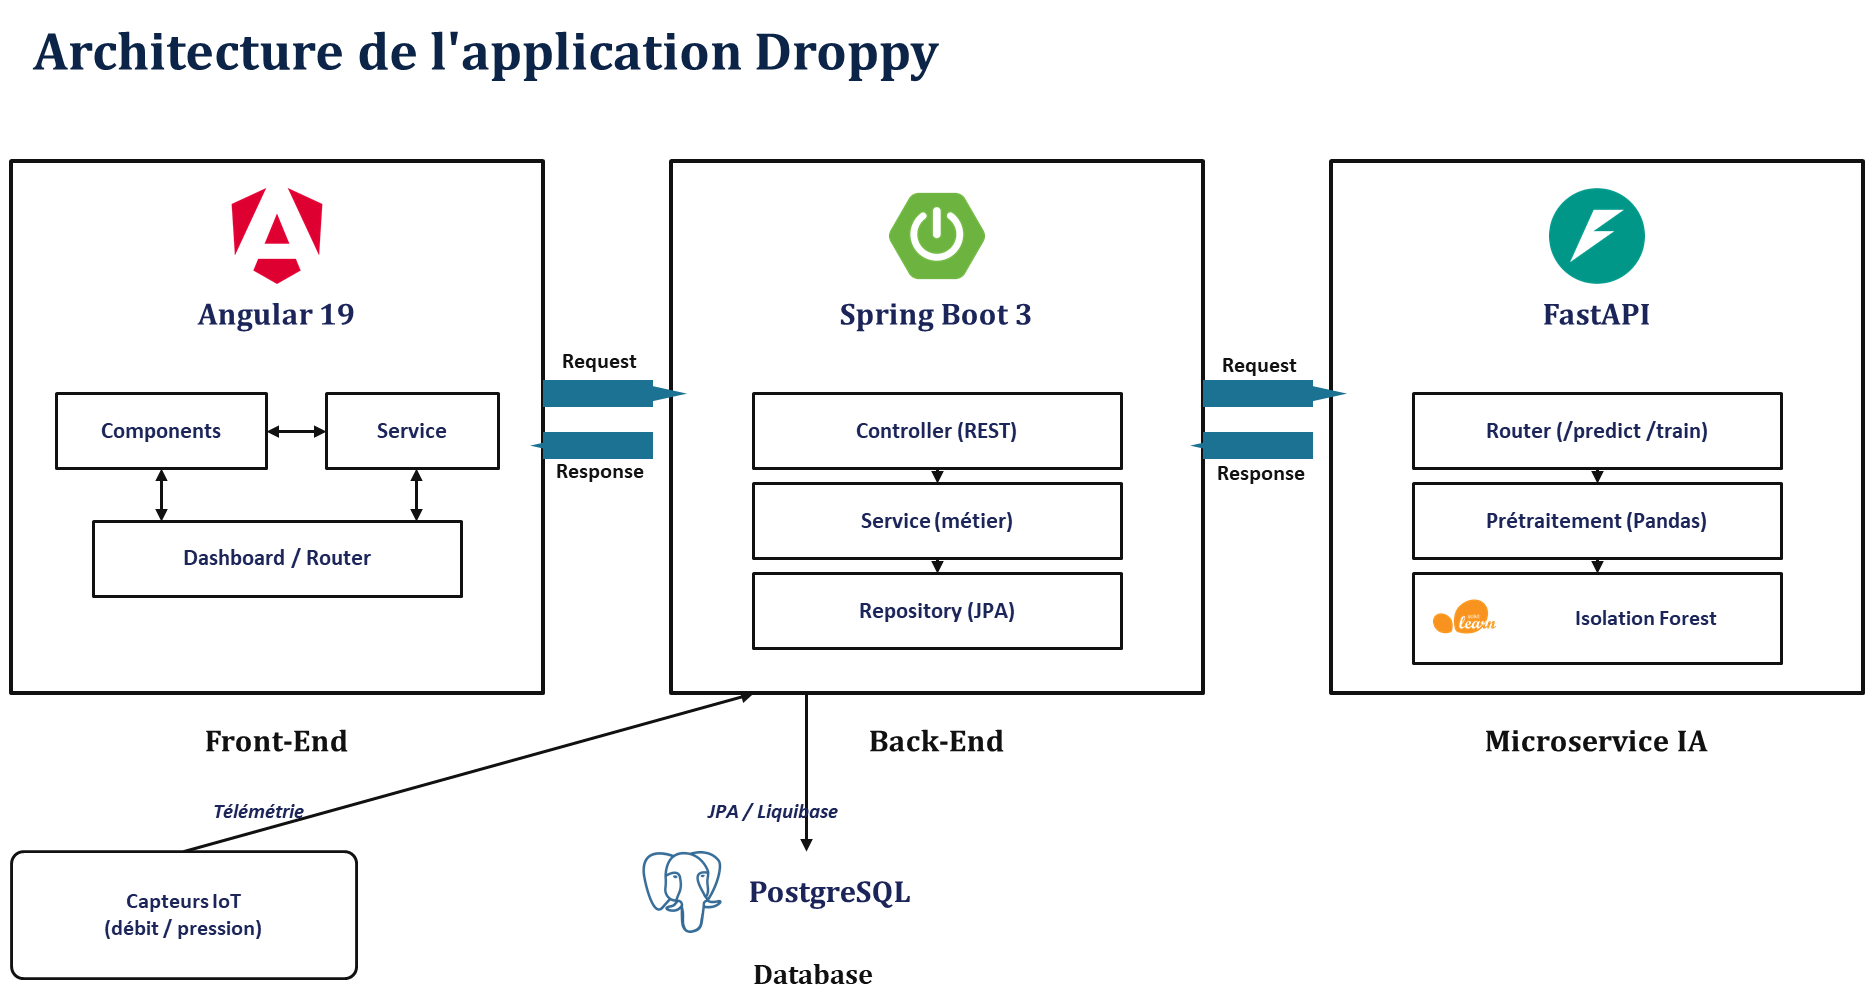
\includegraphics[width=0.95\textwidth]{images/architecture (2).png}
    \caption{Architecture globale de la solution Droppy}
    \label{fig:architecture-globale}
\end{figure}

Cette architecture permet de découpler l'interface, la logique métier et les
traitements d'intelligence artificielle, tout en conservant un point
d'orchestration central.


% =============================================================================
% 3.3 CAS D'UTILISATION
% =============================================================================

\section{Modélisation fonctionnelle}

Le diagramme de cas d'utilisation présente les principales interactions entre
l'utilisateur et la solution Droppy.

L'opérateur constitue l'acteur principal du système. Il utilise le dashboard
pour consulter les anomalies, visualiser les données, demander une analyse,
consulter les prévisions et traiter les anomalies détectées.

Les traitements automatiques sont également représentés afin de montrer que
certaines opérations, notamment l'analyse périodique des dispositifs, sont
déclenchées sans intervention directe de l'utilisateur.

\begin{figure}[H]
    \centering
    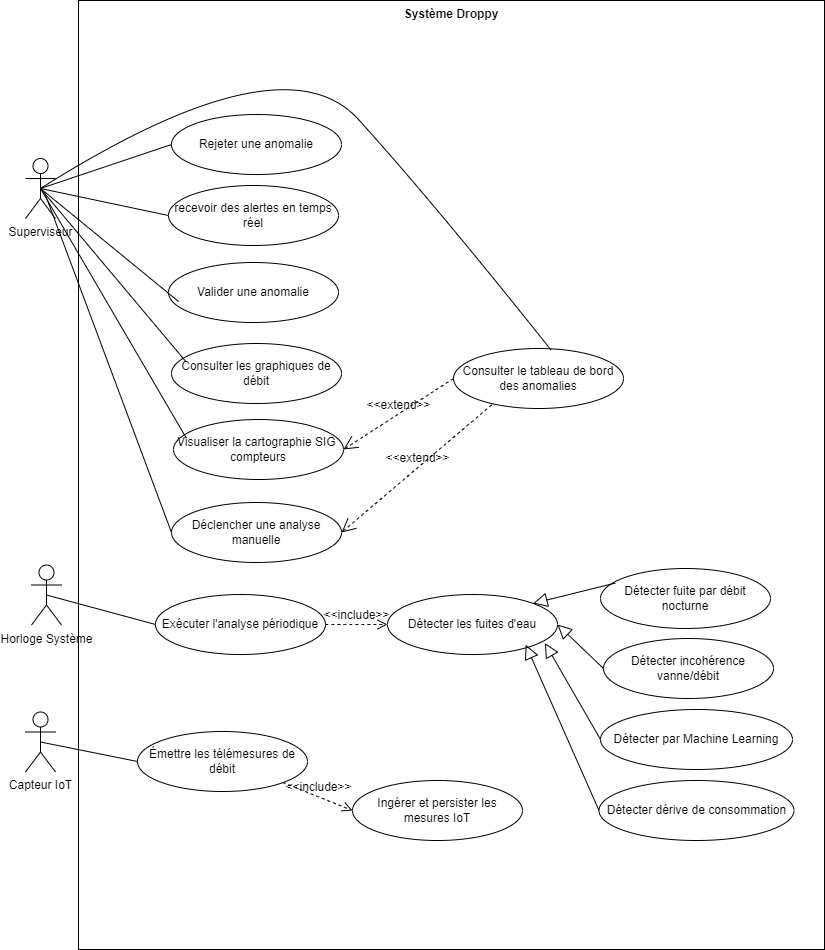
\includegraphics[width=\textwidth]{images/usecase.drawio.png}
    \caption{Diagramme de cas d'utilisation de Droppy}
    \label{fig:use-case-droppy}
\end{figure}

Ce modèle fournit ainsi une vue fonctionnelle synthétique des principales
interactions avec la plateforme.


% =============================================================================
% 3.4 MODELISATION DYNAMIQUE
% =============================================================================

\section{Modélisation dynamique}

Les diagrammes de séquence permettent de représenter les échanges entre les
différents composants lors de l'exécution des scénarios principaux de Droppy.

Deux scénarios ont été retenus : la détection d'une anomalie et la prévision
de consommation.


% -----------------------------------------------------------------------------
% 3.4.1 DETECTION
% -----------------------------------------------------------------------------

\subsection{Détection d'une anomalie}

Le premier scénario représente le processus de détection d'une anomalie.
L'analyse est déclenchée par le scheduler puis orchestrée par le Core Service,
qui sollicite le microservice FastAPI.

\begin{figure}[H]
    \centering
    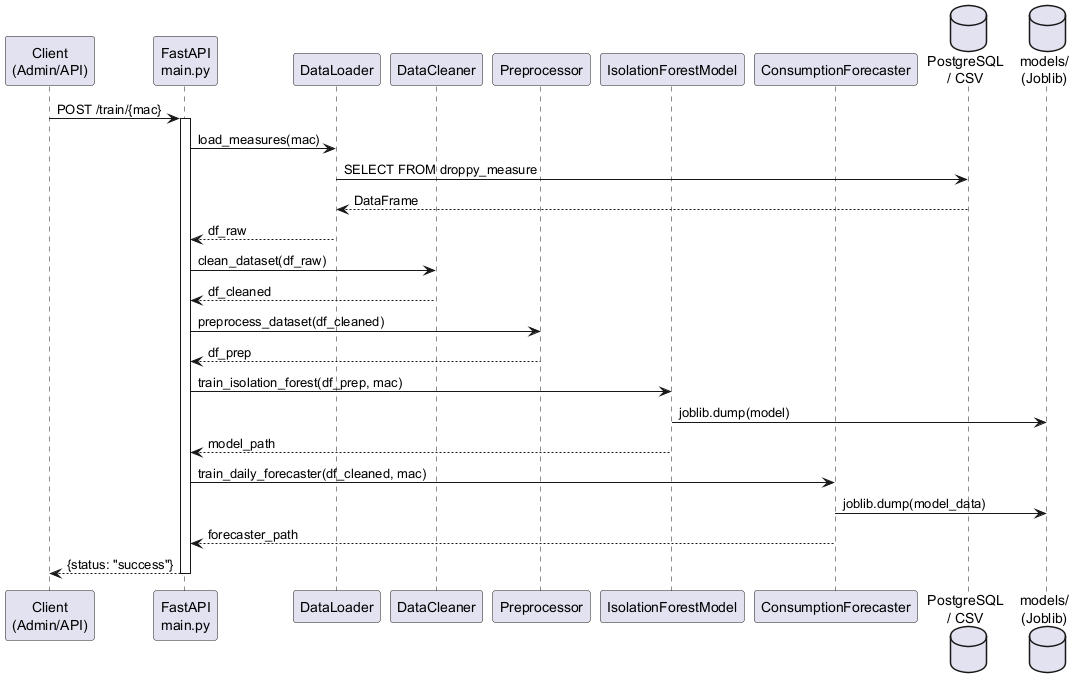
\includegraphics[width=\textwidth]{images/sequence_train.png}
    \caption{Séquence de détection d'une anomalie}
    \label{fig:sequence-detection}
\end{figure}

Le résultat retourné par le service IA est traité par Spring Boot avant
d'être enregistré et transmis au dashboard lorsque cela est nécessaire.


% -----------------------------------------------------------------------------
% 3.4.2 PREVISION
% -----------------------------------------------------------------------------

\subsection{Prévision de consommation}

Le second scénario décrit la demande d'une prévision depuis le dashboard.
La requête traverse le Core Service avant d'être transmise au microservice
FastAPI, qui exécute le modèle de prévision.

\begin{figure}[H]
    \centering
    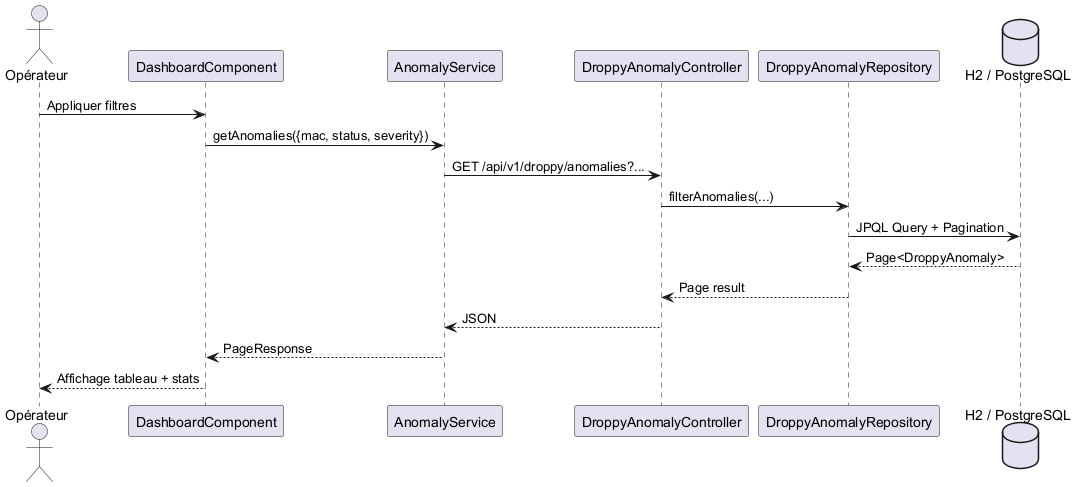
\includegraphics[width=\textwidth]{images/sequence_get.png}
    \caption{Séquence de prévision de consommation}
    \label{fig:sequence-prevision}
\end{figure}

Le résultat est ensuite retourné au dashboard afin d'être présenté à
l'opérateur sous une forme graphique.


% =============================================================================
% 3.5 DIAGRAMME DE CLASSES
% =============================================================================

\section{Modélisation statique}

Le diagramme de classes présente la structure des principaux éléments du
Core Service et leurs relations.

La conception suit une séparation des responsabilités entre les contrôleurs,
les services métier, les repositories et les entités persistantes. La classe
\texttt{DroppyAnomaly} constitue l'entité centrale pour la représentation et
le suivi des anomalies détectées.

\begin{figure}[H]
    \centering
    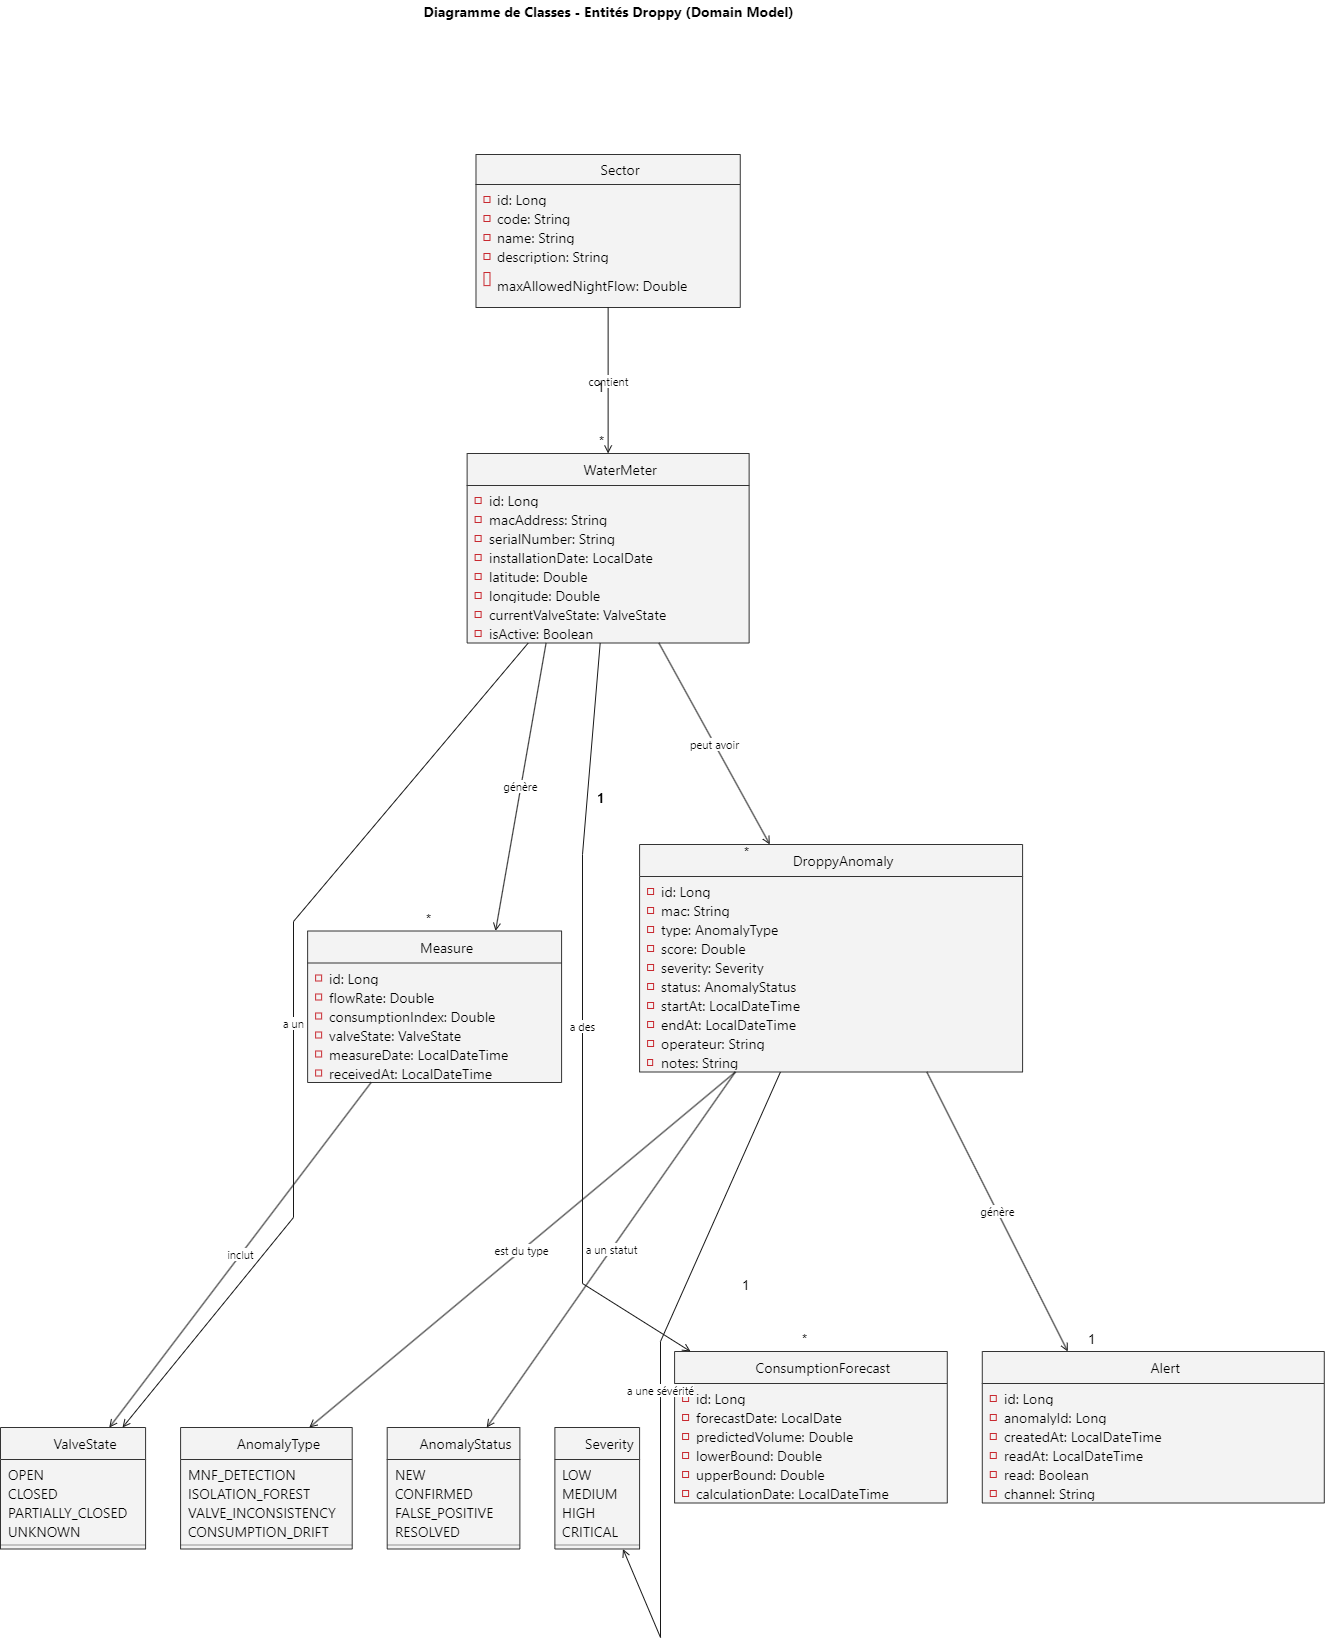
\includegraphics[width=\textwidth]{images/class.drawio.png}
    \caption{Diagramme de classes principal de Droppy}
    \label{fig:diagramme-classes}
\end{figure}

Cette organisation permet de maintenir une séparation claire entre
l'exposition des API, la logique métier et l'accès aux données.
\clearpage

% 
\section{Conclusion}

Ce chapitre a présenté la conception de Droppy à travers plusieurs vues
complémentaires.

L'architecture globale a permis de définir l'organisation des principaux
services, tandis que les diagrammes de cas d'utilisation et de séquence ont
permis de représenter les interactions et les scénarios essentiels. Le
diagramme de classes a décrit la structure statique du système et le diagramme
de déploiement a présenté son organisation dans l'environnement d'exécution.

Cette conception constitue la base de la réalisation technique présentée dans
le chapitre suivant.